\documentclass[12pt]{article}

\usepackage{geometry}
\geometry{letterpaper, total={7in, 10in} }
\usepackage{setspace}
\setstretch{1.2}
\usepackage{booktabs}
\usepackage{graphicx}
\usepackage{verbatim}
\usepackage{appendix}

\title{UGA Data Science Competition 2021}
\author{Ayush Kumar, Chloe Phelps, Faisal Hossain, Nicholas Sung}
\date{April 15, 2021}

\begin{document} 
	
	\maketitle
	\tableofcontents
	\newpage
	
	\section{Exploratory Data Analysis and Preprocessing}
	
	\subsection{Summary Statistics for Continuous Variables}
	
	We begin our exploratory data analysis by looking into the data, and determining the type of the data for each column. For continuous numerical data, we want to visualize the distribution using histograms as well as taking a look at the following summary statistics: mean, standard deviation, the minimum and the maximum. For the categorical data we want to take a look at the possible categories, and the frequency of each category. 
	
	Using pandas and the information sheet here are the numerical variables: 
	

	\begin{tabular}{lrrrrrrrr}
\toprule
{} &    count &          mean &           std &           min &           25\% &           50\% &            75\% &            max \\
\midrule
tot\_credit\_debt                    &  20000.0 &  94563.702530 &  23546.443862 &   2367.430000 &  78743.750000 &  94670.630000 &  110329.335000 &  188890.960000 \\
avg\_card\_debt                      &  20000.0 &  14088.235475 &   9314.495936 &   2363.120000 &  11321.502500 &  13243.750000 &   15196.060000 &   99999.000000 \\
credit\_age                         &  20000.0 &    296.697000 &     61.711702 &     54.000000 &    255.000000 &    297.000000 &     339.000000 &     545.000000 \\
credit\_good\_age                    &  20000.0 &    149.771750 &     34.016476 &     21.000000 &    127.000000 &    150.000000 &     172.000000 &     296.000000 \\
non\_mtg\_acc\_past\_due\_12\_months\_num &  20000.0 &      0.111350 &      0.433890 &      0.000000 &      0.000000 &      0.000000 &       0.000000 &       4.000000 \\
non\_mtg\_acc\_past\_due\_6\_months\_num  &  20000.0 &      0.027400 &      0.171903 &      0.000000 &      0.000000 &      0.000000 &       0.000000 &       2.000000 \\
mortgages\_past\_due\_6\_months\_num    &  20000.0 &      0.030200 &      0.171142 &      0.000000 &      0.000000 &      0.000000 &       0.000000 &       1.000000 \\
credit\_past\_due\_amount             &  20000.0 &    329.287867 &   2073.899357 &      0.000000 &      0.000000 &      0.000000 &       0.000000 &   32662.980000 \\
inq\_12\_month\_num                   &  20000.0 &      1.762700 &      1.740816 &      0.000000 &      0.000000 &      1.000000 &       3.000000 &      10.000000 \\
card\_inq\_24\_month\_num              &  20000.0 &      3.409600 &      2.926697 &      0.000000 &      1.000000 &      3.000000 &       5.000000 &      18.000000 \\
card\_open\_36\_month\_num             &  20000.0 &      0.163050 &      0.386099 &      0.000000 &      0.000000 &      0.000000 &       0.000000 &       2.000000 \\
auto\_open\_ 36\_month\_num            &  20000.0 &      0.141000 &      0.349607 &      0.000000 &      0.000000 &      0.000000 &       0.000000 &       2.000000 \\
uti\_card                           &  20000.0 &      0.503157 &      0.109354 &      0.065120 &      0.429611 &      0.502800 &       0.577412 &       0.969289 \\
uti\_50plus\_pct                     &  20000.0 &      0.511007 &      0.113456 &      0.033749 &      0.435171 &      0.509922 &       0.588418 &       0.988964 \\
uti\_max\_credit\_line                &  20000.0 &      0.507629 &      0.108624 &      0.005174 &      0.433550 &      0.507193 &       0.581376 &       1.000000 \\
rep\_income                         &  18430.0 &  75499.511666 &  16361.955146 &  12000.000000 &  64000.000000 &  75000.000000 &   86000.000000 &  150000.000000 \\
\bottomrule
\end{tabular}

	
	By looking at the descriptive statistics we can see if there are any major outliers, and determine how we can use these variables in our data. We see that minimum and maximum values for many of the continuous variable are very extreme for Total Credit Debt, Average Credit Debt, and Credit past due amount. We also see that many variables seem to have very similar distributions, which may be a problem in regards to multi-collinearity. To investigate this we can create a correlation matrix and re-scale certain variables to try to preserve information, while combating multi-collinearity. 
	
	\begin{center}
			\includegraphics[scale = 0.15]{../notebooks/dist.png}
	\end{center}


	Looking at the histogram gives us a better picture of the distributions of the variables because it allows us to visualize the shapes of the variables. We can see that the outliers for Average Credit Debt are seriously impacting the distribution in comparison to Total Credit Debt. This visualization also allows us to look at some variables which by their description seem to be numerical, but display behavior that is more characteristic of categorical variables. Variables like the number of mortgages past due or non-mortgages past due would be better suited to being dummy variables rather than continuous ones. 
	
	\begin{center}
		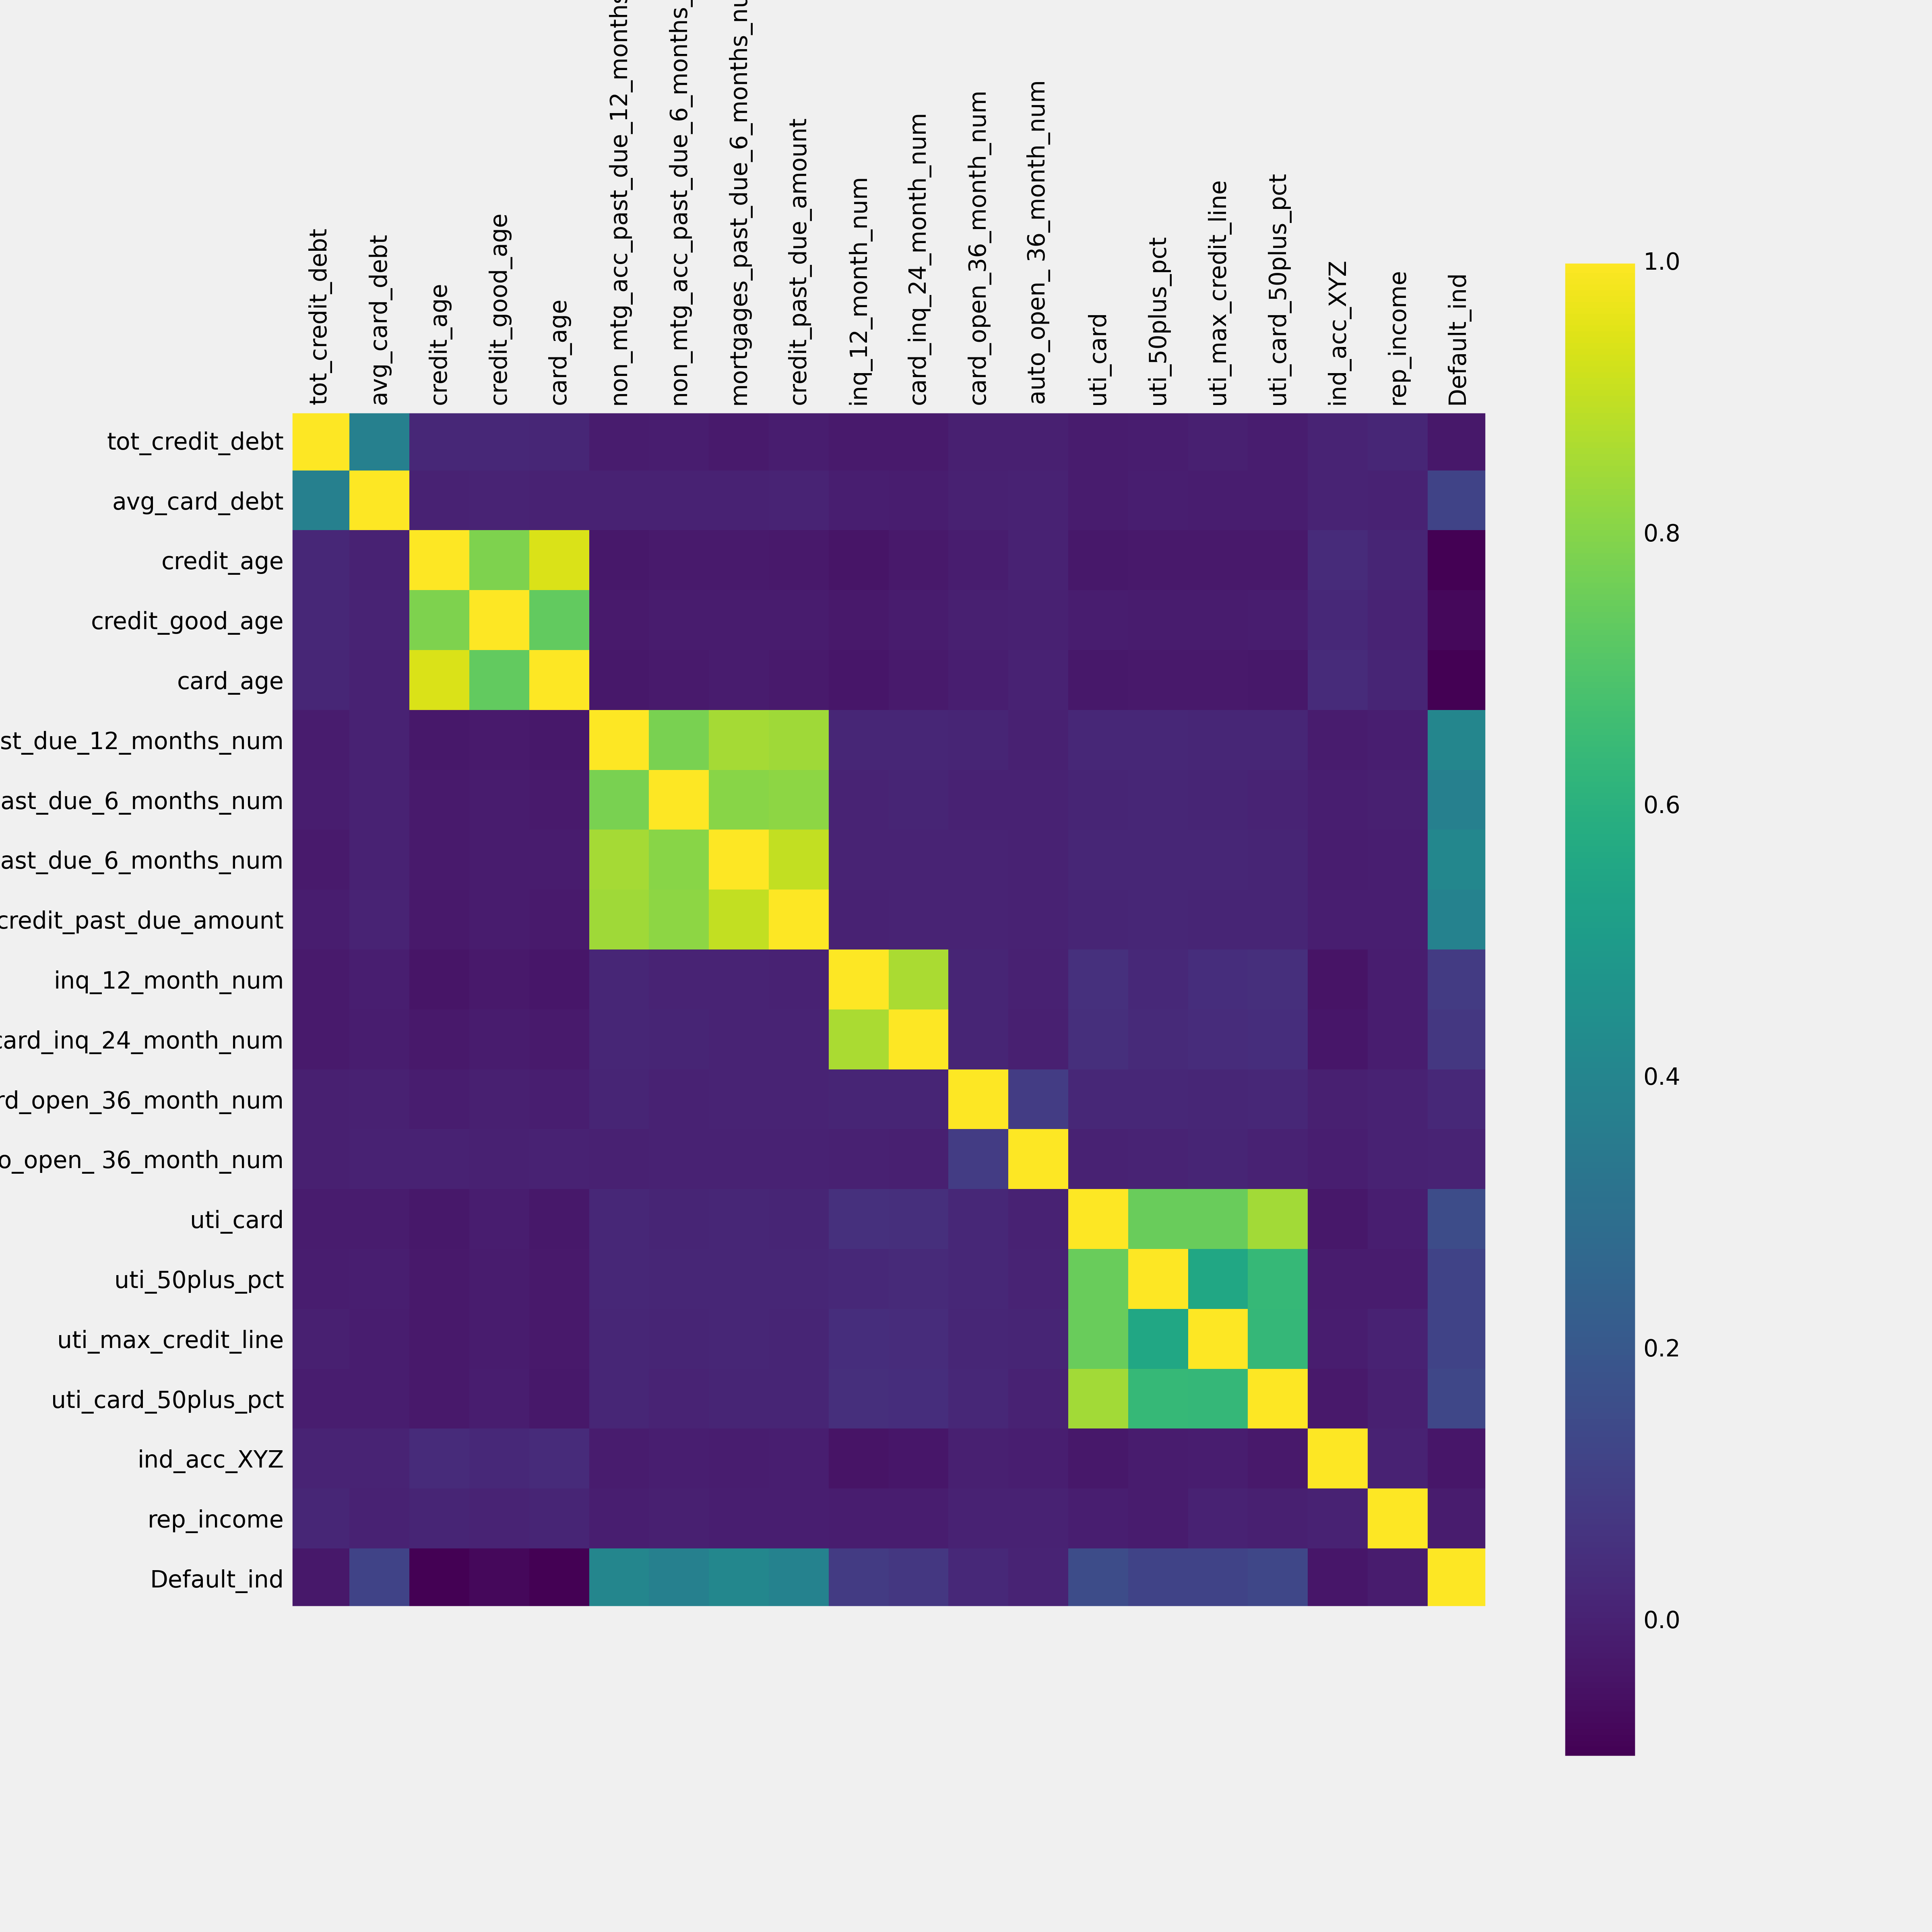
\includegraphics[scale = 0.3]{../notebooks/CorMat.png}
	\end{center}
	
	Taking a look at the correlation matrix we can see multiple points of high collinearity between variables that are similar in nature due to the time that they are recorded or other inherent similarities. Based on this correlation matrix we can see that some of the variables may need to be rescaled to preserve as much information as possible, but bring down the high collinearity. Another approach would be to carry on with all the variables and not put too much stock into the individual variable t-tests and instead focus on joint F-tests and ensure that the variables are being properly captured. 
	
	\subsection{Summary Statistics for Categorical Variables}
	
	\begin{center}
		\includegraphics[scale=0.15]{../notebooks/counts.png}
	\end{center}
	
	We can take a look at the counts and the relative frequencies for the variables and make some observations. For many of these variables it would be wise 
	to make multiple dummy variables to allow for better predictive models. States and card\_open\_36\_month\_num should be split into multiple variables for the models. The other variables are either in a form that already mimics a dummy variable, or they can easily be converted into 0 or 1 dummy variables because given the small frequency numbers higher than one appear it would be superfluous to have multiple dummy variables for the different variables. Further analysis is required for the State dummy variables because there need to be substantial differences between the different states to add them as dummy variables. 
	
	The analysis we choose for adding state dummy variables is to simply take a look a random sample of observations and plot a subset of two variables that are representative of the data available and plot them by state. Based on the graphs on page 5 we can see that there are some patterns however weak in the data and we should take them into account when building the model. The significance of the state dummy variables can be assessed at a later time after the models have been built. 
	
	\begin{center}
		\includegraphics[scale = 0.15]{../notebooks/states.png}	
	\end{center}
	
	\subsection{Model Selection}
	
	In addition to the Logistic Regression we were asked to choose between a Feed-Forward Neural Network, a Random Forest Classifier, or XGBoost. Due to the high number of possible interaction effects as well as the high number of continuous variables our team has opted to use the Feed-Forward Neural Network. These networks can be useful because they allow for a very high number of interaction effects without extensive testing. We will use a sigmoid function as our last response function to ensure the model output is similar to the output of the logistic regression.
	
	Another challenge in model building will be the relatively low number of observations that do default on their credit debt. This makes it extraordinarily difficult to make sure our models are genuine improvements over the baseline model of predicting 0 for every observations. This baseline model has an accuracy of 92\% so it will be important that we do not over-depend on accuracy as a measure of model fit. Precision, recall, and f1-scores will be much better indicator of model fit, and should be used when tuning hyper-parameters. 
	
	\subsection{Preprocessing Transforms}
	
	We will be using data in numpy arrays, but first we must overcome some of the challenges of this approach. We must have numerical data for every observation, and there can be no missing values or the logistic regression model will not function properly. Our \verb|load_data(path: String): X, y| function will conduct the following transforms on the data to prepare it for model use. 
	
	\begin{enumerate}
		\item Import data from a csv into a pandas dataframe
		\item Impute missing numeric values using the expected value of a column
		\item Turn the following rows into dummy variables based on various levels: States, non\_mtg\_*, card\_open\_*, auto\_open\_*
		\item Split the dataset into X - the data matrix and y - the response column
	\end{enumerate}
	
	\section{Logistic Regression Model}
	
	\subsection{Baseline Model}
	
	Using the preprocessed data as discussed above we trained a logistic regression model from sklearn without tuning any hyper parameters. 
	The following were the model coefficients and performance statistics on the testing dataset. 
	

	\begin{tabular}{c|c|c|c|c|c}
	\hline
			& 		& 	precision &  recall  & f1-score   & support \\ \hline
			
			&  0.0	  &		0.93 &     0.99   &  0.96    &  4599 \\ \hline
			&  1.0    &		0.72 &     0.20   &   0.31   &    401 \\ \hline
			
			accuracy & & & &                       					0.93     & 5000 \\ \hline
			macro avg  & &   				0.83   &   0.60  &    0.64  &    5000  \\ \hline
			weighted avg  & &   			0.92   &   0.93  &    0.91   &   5000 \\ \hline
	\end{tabular}					

	The coefficients and interpretation of them is available in Appendix A. The scores can help us assess model performance. The initial news seems to be good with an overall accuracy of 93\%, but this is only marginal better than baseline model. The precision of the model is also ok with a score of 0.92. This means that of all the observations identified by the model as clients who will default we are correct around 72\% of the time. The worrisome part of this model is the recall. A recall of 0.20 implies that we are missing nearly 4/5 of all clients who will end up defaulting. In other words this model is extremely good at identifying that a client will NOT default, but in the process misses a lot of clients who will default. This is all assuming a decision boundary of 0.5, which we will be optimizing. If the firm wants to minimize default risk it will have to increase the decision boundary, and if a firm wants to maximize the amount of credit they are lending the decision boundary should be decreased. Our team believes that defaults are much more costly, and we should try to tune the decision boundary in  way that is beneficial to the end goal of reducing defaults. 
	
	It should also be noted that for a logistic regression we can directly interpret the variables and the effect they will have on the overall model. This will be discussed in greater detail in the explanation section of the report.

	\subsection{Tuning Decision Boundary}
	
	We will be using an algorithm that tries to maximize recall while ensuring that precision does not fall below a certain level. We will be able to test multiple values of the level we want to let the precision fall down to. We will be using a variable learning rate that decreases in a reciprocal fashion every iteration. We will be updating the decision boundary by subtracting the previous boundary times the learning rate for that iteration. 
	
	$$ \eta_{t+1} = \eta_0/t $$ 
	
	$$ threshold_{t+1} = threshold_t*eta_t $$
	
	This is to ensure that we arrive at a decision boundary that converges. The method signature is as follows: \verb|tune_threshold(y, yhat, eta, plev): Double|. The plev is the level of precision we are willing to go down to and by generating many thresholds at different levels of precision we will be able to generate graphs of where the ideal decision boundary may lie. We assume an initial threshold of 0.5 and we will tune from there. Using this algorithm our group tested every precision between 0 and 1 with an increment of 0.1 and plotted the results. 
	
	\begin{center}
		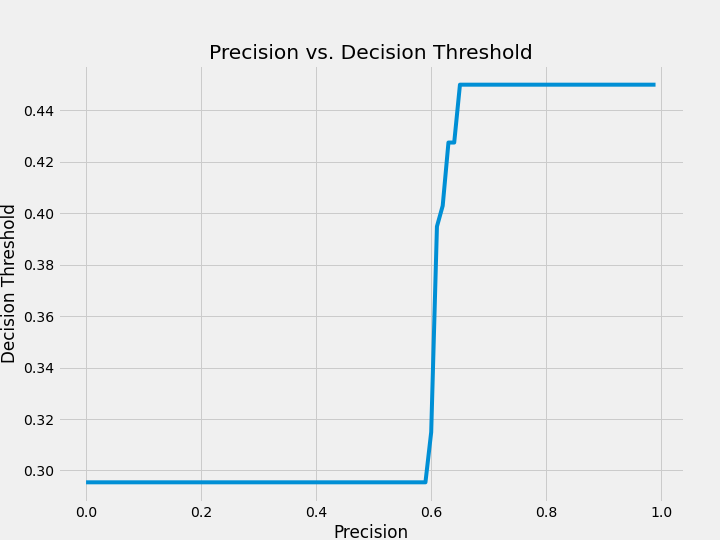
\includegraphics[scale = 0.4]{../notebooks/precisionvsthreshold.png}
	\end{center}
	
	Based on the results it seems that precision is not very sensitive for most values between 0.6 and 1.0 and between 0.0 and 0.6. This behavior is indicative of the precision recall trade-off in our model. To have an substantial gains of recall we would have to expand the number of applications the model will reject be quite a heavy amount. We can see that in the following precision and recall curve for our logistic regression model. 
	
	\begin{center}
		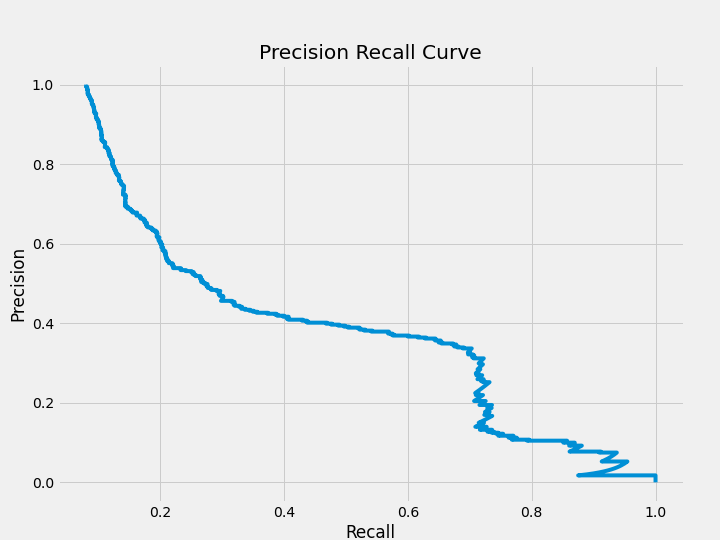
\includegraphics[scale=0.4]{../notebooks/pr_curve_lr.png}
	\end{center}

	We see much of the same behavior we expected from our initial analysis of the precision-threshold curve. Around a precision of 0.5 we begin to see a substantial gain of recall at the cost of precision. Based on this our team recommends using a decision boundary based on preserving a precision of 0.5 and attempting to get much recall as we can. This will reduce our overall accuracy, but ensure that we catch more people who are likely to default on their credit loans minimizing the risk to the firm. This decision boundary for precision level of 0.5 happens to be 0.1514. Here is a summary of model fit after using this decision boundary on the test dataset. The decision boundary was tuned using the validation dataset. 
	
	
	\begin{tabular}{c|c|c|c|c|c}
	\hline
				& 		& 	precision &  recall  & f1-score   & support \\ \hline
	
				&  0.0	&		0.95 &     0.98   &  0.96   &  4599 \\ \hline
				&  1.0  &		0.61 &     0.37   &  0.46   &   401 \\ \hline
	
	accuracy    & & & &                       		  0.93   &   5000 \\ \hline
	macro avg   & &   			0.78   &   0.67  &    0.71   &   5000  \\ \hline
	weighted avg  & &   		0.92   &   0.93  &    0.92   &   5000 \\ \hline
	\end{tabular}	
	 
	
	When using the testing dataset we have greatly improved the recall of our model, while sacrificing a small amount of precision. This means the firm can still be extremely confident in knowing the model will rarely classify a non-defaulter as someone who will default, and will be assuming less risk in terms of trying to catch as many defaulters as possible. 
	
	
	\section{Feed Forward Neural Network Model}
	
	\subsection{Initial Model}
	
	The feed-forward neural network was chosen because of its ability to capture nonlinear interaction effects that may exist between variables. Some downsides of this type of network include its black-box nature, the cost of training, and the possibility of arriving at a local optimum rather than a global optimum. We must take extreme care to ensure that we do not accidentally converge at an incorrect minimum. Our model will be using a single hidden layer with a relu activation function and a single output node of with a sigmoid activation function. We will start with a model with a number of hidden nodes equal to the number of input features and a loss based on binary cross entropy. 
	
	\begin{tabular}{c|c|c|c|c|c}
	\hline
	& 		& 	precision &  recall  & f1-score   & support \\ \hline
	
	&  0.0	&		0.93 &     0.99   &  0.96   &  4599 \\ \hline
	&  1.0  &		0.76 &     0.19   &  0.31   &   401 \\ \hline
	
	accuracy    & & & &                       		  0.93   &   5000 \\ \hline
	macro avg   & &   			0.85   &   0.59  &    0.64   &   5000  \\ \hline
	weighted avg  & &   		0.92   &   0.93  &    0.91   &   5000 \\ \hline
	\end{tabular}
	
	Our initial model has a similar problem to the original logistic regression, but before be begin tuning the decision curve, we can make adjustments to the model architecture. 
	
	
	\subsection{Model Stability}
	
	To ensure model stability we are training our feed forward neural network 100 times over 100 epochs and then checking the distribution of precision and recall scores to ensure that our model is stable. 
	
	\begin{center}
		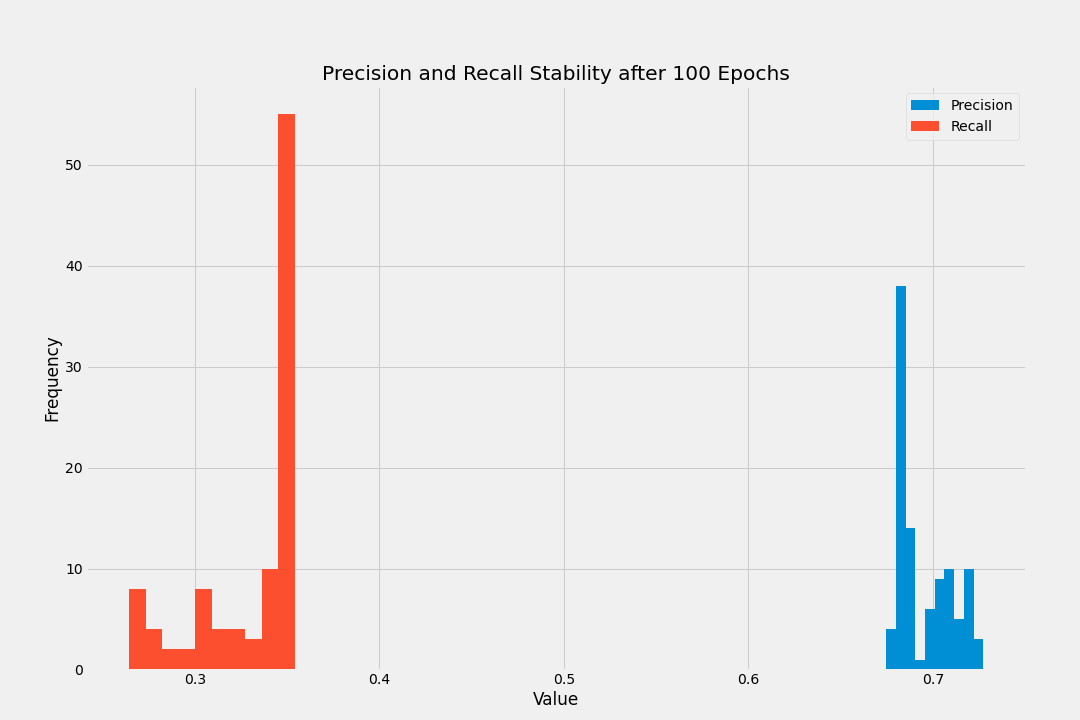
\includegraphics[scale=0.4]{../notebooks/StableNetwork.png}
	\end{center}
	
	After running 100 networks for 100 epochs we find that we have indeed reached a stable network. Furthermore there is even more good news as we can see that recall scores are on average much higher than the recall scores from the logistic regression. Here is the performance report for a network trained for 100 epochs. 
	
	\begin{tabular}{c|c|c|c|c|c}
		\hline
		& 		& 	precision &  recall  & f1-score   & support \\ \hline
		
		&  0.0	&		0.95 &     0.99   &  0.97   &  4599 \\ \hline
		&  1.0  &		0.69 &     0.34   &  0.46   &   401 \\ \hline
		
		accuracy    & & & &                       		  0.93   &   5000 \\ \hline
		macro avg   & &   			0.82   &   0.67  &    0.71   &   5000  \\ \hline
		weighted avg  & &   		0.92   &   0.93  &    0.92   &   5000 \\ \hline
	\end{tabular}
	
	This is extremely promising and is almost outperforming our tuned logistic regression model without taking a look at the precision recall curve. The next step in analysis for the feed forward network is to of course try to tune the decision boundary to maximize recall while making minimum sacrifices to our precision. 
	
	\subsection{Tuning Model Width}
	
	
	The first item to consider is the complexity of the model. We may be over or under parameterize, and this can be tuned by simply changing the number of elements in the hidden node. Here are graphs of precision, recall, and accuracy, as we change the number of nodes in the hidden layer. 
	
	
	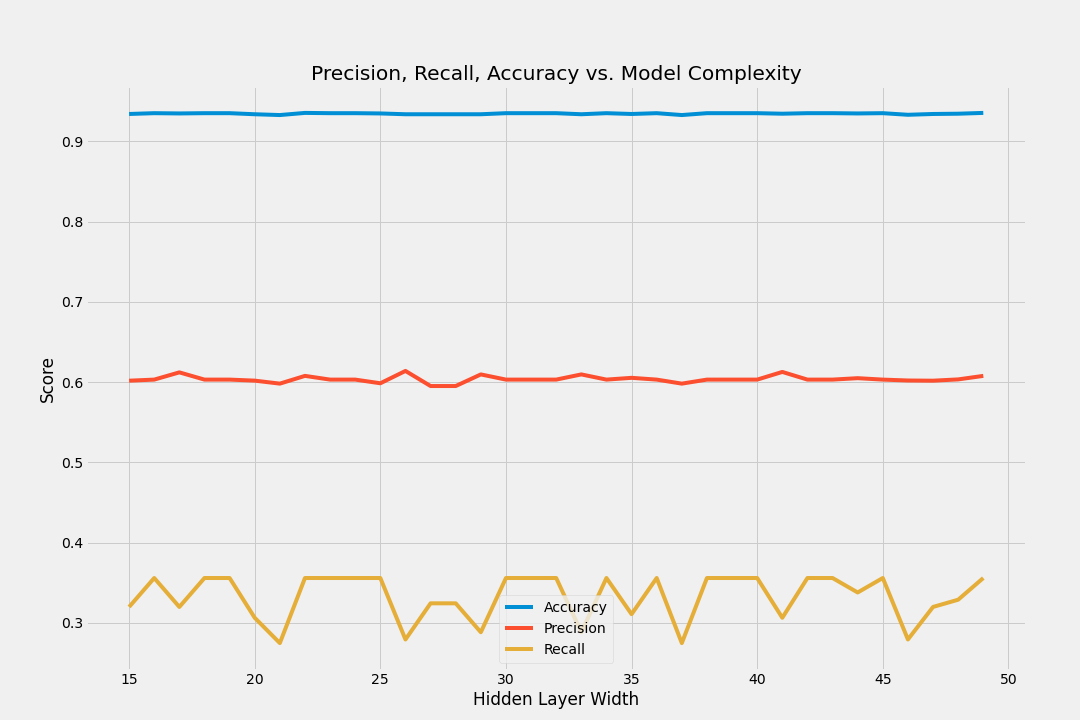
\includegraphics[scale=0.4]{../notebooks/nn_width.png}
	
	It seems that there is no tangible benefit to increasing the model complexity past the point that we currently have it. Our metrics seem to be very stable at their level. 
	
	
	\subsection{Tuning Decision Boundary }
	
	\begin{center}
		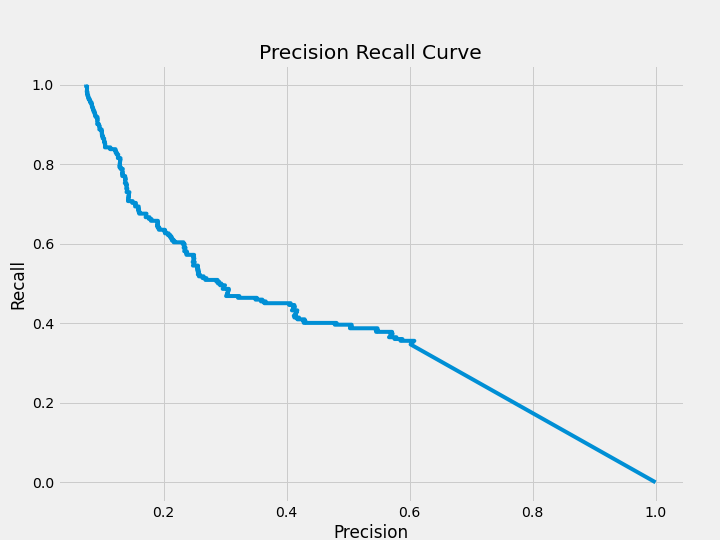
\includegraphics[scale=0.3]{../notebooks/pr_curve_nn.png}
		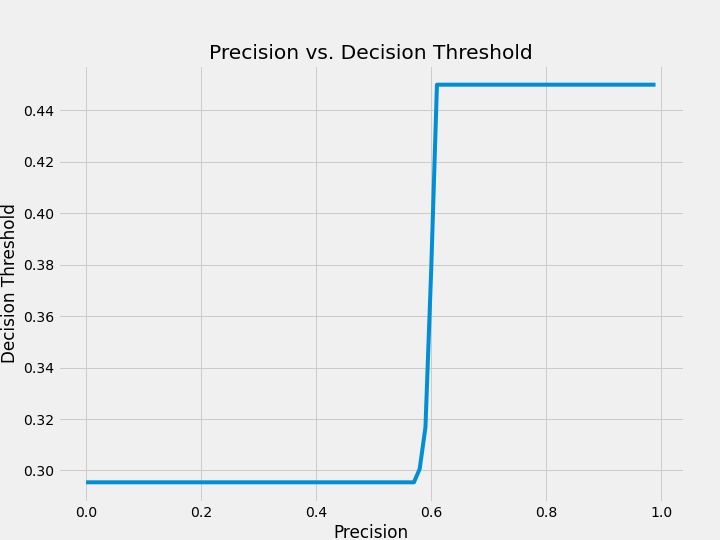
\includegraphics[scale=0.3]{../notebooks/precisionvsthreshold_nn.png}
	\end{center}
	
	Taking a look at the two graphs  we can see very similar behavior when it comes to the Precision vs. Threshold graph in comparison to the logistic regression model, but the precision recall curve seems to be much more promising when it comes to our neural network. Looking at the curve the tuning precision of 0.55 seems to be a good sacrifice as the precision recall curve is quite steep. This yields a decision boundary of 0.2602 and the following evaluation: 
	
	\begin{tabular}{c|c|c|c|c|c}
		\hline
		& 		& 	precision &  recall  & f1-score   & support \\ \hline
		
		&  0.0	&		0.95 &     0.98   &  0.96   &  4599 \\ \hline
		&  1.0  &		0.62 &     0.38   &  0.47   &   401 \\ \hline
		
		accuracy    & & & &                       		  0.93   &   5000 \\ \hline
		macro avg   & &   			0.78   &   0.68  &    0.72   &   5000  \\ \hline
		weighted avg  & &   		0.92   &   0.93  &    0.92   &   5000 \\ \hline
	\end{tabular}
	
	Beyond this point improving recall requires a much greater sacrifice in precision and it will not be in the firm's interest to go beyond this decision boundary. 
	
	\subsection{Comparison with Logistic Regression}
	
	When we compare the best statistics we were able to get from both the neural network and logistic regression after tuning the decision boundary we arrive at models that perform much the same in most regards. In fact the differences between the two models end up being so small that they could not be said to be statistically significant; however, when it comes to untuned models the neural network far outperforms the logistic regression model, and the untuned version may in fact be a better compromise than the tuned version of the network. For this reason, the model our team recommends for further study and potential future use is the stable, untuned feed-forward neural network. The disadvantage of this model is the high training times, and the potential black box nature. To effectively arrive at reasoning we will have to run multiple observations through the model and observe differences, there is no direct interpretation of the results that can be had from the neural network coefficients and parameters. 
	
	
	\section{Future Decision Making}
	
	We will be using a simple but effective approach to explain the decision making process of neural network. This process involves running the mean values through the network, and then making a single change to a single observation and then comparing the results. By doing this for every variable between a given consumer and the mean consumer we can come up with explanations for the strongest reasons a consumer was accepted or denied for a credit card with the firm. We will use this approach for all consumers to try to answer the question of bias with previous consumers at our branch. 
	

	\subsection{Explaining Model Decisions}
	Using the approach of tracking changes from the mean we must first come up with the mean probability for someone who is precisely average. Here we can see that the mean probability is 0.2139 this can be seen as the average risk. Assuming we know nothing about a customer this is the risk that they will default on their credit debt. By tracking changes one at a time and comparing it one at at time we can come up with analysis on how a decision was made. Take these sample observations on page 14 as an example.
	 Person45 defaulted on their payments, and person1 did not. We can take a look at the observations and see that Person45 was categorized as someone who would default because most of their observations were around the mean, but because of their high total credit debt and credit age they were presumed to be someone with a much higher risk to the firm. 
	 Person1 also has a high total credit debt and low credit age, but the rest of their observations are near the mean or below the mean which substantially lowers their risk to the firm. For this reason person1's credit was approved by the model, and person45's credit was not approved by the model. 
	
	\begin{tabular}{lrr}
\toprule
{} &      Person45 &   Person1 \\
\midrule
tot\_credit\_debt                         &  1.000000e+00 &  0.514523 \\
avg\_card\_debt                           &  4.437685e-03 &  0.137980 \\
credit\_age                              &  3.770228e-01 &  0.372324 \\
credit\_good\_age                         &  2.526338e-01 &  0.257978 \\
card\_age                                &  3.722641e-01 &  0.383290 \\
mortgages\_past\_due\_6\_months\_num         &  2.138428e-01 &  0.213843 \\
credit\_past\_due\_amount                  &  3.349119e-02 &  0.033491 \\
inq\_12\_month\_num                        &  1.915515e-01 &  0.200272 \\
card\_inq\_24\_month\_num                   &  1.846877e-01 &  0.196563 \\
uti\_card                                &  2.094540e-01 &  0.210985 \\
uti\_50plus\_pct                          &  2.102203e-01 &  0.211625 \\
uti\_max\_credit\_line                     &  2.107638e-01 &  0.210582 \\
uti\_card\_50plus\_pct                     &  2.099449e-01 &  0.211877 \\
ind\_acc\_XYZ                             &  2.188845e-01 &  0.209320 \\
rep\_income                              &  5.187532e-25 &  0.000000 \\
Default\_ind                             &  2.143294e-01 &  0.213067 \\
FL                                      &  2.130757e-01 &  0.213076 \\
SC                                      &  2.138326e-01 &  0.213833 \\
LA                                      &  2.152982e-01 &  0.215298 \\
GA                                      &  2.134444e-01 &  0.213444 \\
MS                                      &  2.144244e-01 &  0.214424 \\
NC                                      &  2.138411e-01 &  0.213841 \\
non\_mtg\_acc\_past\_due\_12\_months\_num==2.0 &  2.129159e-01 &  0.212916 \\
non\_mtg\_acc\_past\_due\_12\_months\_num==1.0 &  2.139596e-01 &  0.213960 \\
non\_mtg\_acc\_past\_due\_12\_months\_num==3.0 &  2.139562e-01 &  0.213956 \\
non\_mtg\_acc\_past\_due\_12\_months\_num==4.0 &  2.133930e-01 &  0.213393 \\
non\_mtg\_acc\_past\_due\_6\_months\_num==1.0  &  2.139547e-01 &  0.213955 \\
non\_mtg\_acc\_past\_due\_6\_months\_num==2.0  &  2.130403e-01 &  0.213040 \\
card\_open\_36\_month\_num==1.0             &  2.138993e-01 &  0.213899 \\
card\_open\_36\_month\_num==2.0             &  2.130323e-01 &  0.213032 \\
auto\_open\_ 36\_month\_num==1.0            &  2.139616e-01 &  0.213962 \\
\bottomrule
\end{tabular}

	
	\subsection{Previous Customers \& Bias}
	
	We can use this approach to answer the question do people who an account with the bank have an advantage over people who do not have an account with the bank. One approach would be to create two synthetic datasets one with observations of 0 and another with observations with 1. Since most people do not have accounts with bank we can simply track the difference from the mean rather than do the costly process of trying to run over 5000 observations through our explanation function. Here are the results: 
	
	Average Risk for Normal Customer: 0.2139 
	
	Average Risk for Bank Customer: 0.2069
	
	It seems that there is indeed a difference between the assessed risk for a bank consumer and a normal consumer, but it does not seem to be substantial enough to be deemed significant. We could test the statistical significance by trying to run bootstrap with the neural network architecture and evaluate the distributions of these values multiple times over, but this approach is very computationally expensive and would take many hours on our team's machines. For this reason we are choosing to use our judgment and can say that there does not seem to be a significant difference between the assumed risk of a normal customer or a previous customer at the bank. 
	

	
\end{document}	